\documentclass[reprint,english]{revtex4-1}

% language
\usepackage[utf8]{inputenc}
\usepackage[english]{babel}

% standard setup
\usepackage{physics,amssymb,array}
\usepackage{xcolor,graphicx,hyperref}
\usepackage{tikz,listings,multirow}
\usepackage{subfigure}
\usepackage{enumitem}

% hyperref coloring
\hypersetup{ %
  colorlinks,
  linkcolor={red!50!black},
  citecolor={blue!50!black},
  urlcolor={blue!80!black}}

% lstlisting coloring
\lstset{ %
  inputpath=,
  backgroundcolor=\color{white!88!black},
  basicstyle={\ttfamily\scriptsize},
  commentstyle=\color{magenta},
  language=C++,
  tabsize=2,
  stringstyle=\color{green!55!black},
  frame=single,
  keywordstyle=\color{blue},
  showstringspaces=false,
  columns=fullflexible,
  keepspaces=true}
  
\begin{document}
% titlepage
\title{FYS3155 Machine Learning - Project 1\\Studying The Application of Linear Regression in\\Polynomial Parametrisation of Three-Dimensional Surfaces}
\author{Nils Johannes Mikkelsen}
\date{\today}
\noaffiliation
\begin{abstract}
Three-dimensional surfaces are parametrised using polynomial models with coefficients determined by regressional analysis. Three regression methods are used, Ordinary Least Squares, Ridge and Lasso. No particular favourite is found, but the different methods have strengths and weaknesses depending on their application.
\end{abstract}
\maketitle

All material for project 1 may be found at:\\
{\small\url{https://github.com/njmikkelsen/machinelearning2018/tree/master/Project1}}

% body
\section{Introduction}
To count the number of fields in which linear regression has played a pivotal role in the field's research methods is a fool's errand. In fact, the importance of linear regression cannot be understated. The aim of this project is to study one example in which linear regression is applied: namely polynomial parametrisations of three-dimensional surfaces. More concretely, this project aims to study surfaces \(f=f(x,y)\) whose function values are only available as data sets \(\{(x_i,y_i,f_i)\}\), \(i=1,\ldots,N\). The ideal is to be able to analyse the underlying map \(f(x,y)\) by parametrising it with a polynomial map \(z=z(x,y)\), whose coefficients are to be determined using linear regression.

In other words, the goal of this project is to study the behaviour of linear regression when it is used in conjuction with polynomial parametrisations of surfaces. In order to achieve this, the project looks at two different cases: the \emph{well-studied} Franke's test function and a data-set from \url{https://earthexplorer.usgs.gov/}. The former case serves as an analysis of the applicability of the various linear regression methods, while the latter is included for the purpose of studying a real-world example surface.
\section{Linear Regression}
\subsection{The fundamentals}
The basic idea behind linear regression is to fit a function value \(y=y(\vb{x})\) to some model \(f(\vb{x})\). Mathematically speaking, \(f(\vb{x})\) maps the \(n\)-dimensional input value \(\vb{x}\) to the single-valued estimate \(f(\vb{x})\) of the function value \(y\). The map \(f(\vb{x})\) may itself be composed of a several submaps \(f_j(\vb{x})\). The only requirement is that the main map should be a linear combination of the submaps with coefficients \(\beta_j\), called the model parameters:
\begin{equation}\label{eq:fundamental_linear_regression_equation}
y_i=f(\vb{x}_i)+\varepsilon_i=\beta_1f_1(\vb{x}_i)+\cdots+\beta_Mf_M(\vb{x}_i)+\varepsilon_i
\end{equation}
The added error-term \(\varepsilon_i\) makes the equation an equality. The fundamental assumption of linear regression is that this error-term behaves according to a normal distribution \(N(\mu,\sigma^2)\). Linear regression is concerned with the estimation of the model parameters such that the model \(f(\vb{x})\) is "as close as possible" to \(y\). This vague closeness-terminology is the actually the basis for the existence of different kinds of linear regression methods. This project employs three different kinds of linear regression methods: Ordinary Least Squares (OLS), Ridge and Lasso.

Mathematically speaking, "how close" \(f(\vb{x})\) is to \(y\) is measured using a statistical measure. OLS defines closenes via the Mean Squared Error:
\begin{equation}\label{eq:MSE}
\text{MSE}(y,\vb{x},f)=\sum_{i=1}^N\big(y_i-f(\vb{x}_i)\big)^2
\end{equation}
In addition to OLS's MSE measure, Ridge and Lasso includes an additional penalty term:
\begin{equation}\label{eq:penalty}
\text{penalty}(\lambda,p,\beta)=\lambda\sum_{j=0}^M\abs{\beta_j}^p
\end{equation}
The difference between Ridge and Lasso lies in the value of \(p\): Ridge defines \(p=2\), while Lasso defines \(p=1\).
\subsection{Matrix formulation}
We now introduce the vector quantities
\begin{subequations}
\begin{align}
\vb{y}&=\mqty(y_1&\cdots&y_N)^T\\
\vb{x}&=\mqty(x_1&\cdots&x_n)^T\\
\hat{\beta}&=\mqty(\beta_1&\cdots&\beta_M)^T\\
\vb{\varepsilon}&=\mqty(\varepsilon_1&\cdots&\varepsilon_N)^T
\end{align}
\end{subequations}
Combining equation \eqref{eq:fundamental_linear_regression_equation} for each \(i\in\{1,\ldots,N\}\) into a single column vector we find
\begin{align*}
\mqty(y_1 \\ \vdots \\ y_N)&=\mqty(\beta_1f_1(\vb{x}_1)+\cdots+\beta_Mf_M(\vb{x}_1) \\ \vdots \\ \beta_1f_1(\vb{x}_N)+\cdots+\beta_Mf_M(\vb{x}_N))+\mqty(\varepsilon_1\\\vdots\\\varepsilon_N)\\
\mqty(y_1 \\ \vdots \\ y_N)&=\mqty(f_1(\vb{x}_1)&\cdots&f_M(\vb{x}_1)\\ \vdots & & \vdots \\ f_1(\vb{x}_N)&\cdots&f_M(\vb{x}_N))\mqty(\beta_1 \\ \vdots \\ \beta_M) + \mqty(\varepsilon_1\\\vdots\\\varepsilon_N)\\
\vb{y}&=\hat{X}\hat{\beta}+\vb{\varepsilon}
\end{align*}
Using this matrix formulation of linear regression, the matrix \(\hat{X}\) is commonly refered to as the design matrix of a given model \(f(\vb{x})\).

The next step is to rewrite the statistical measures using the same matrix formulation.
\begin{align}
\text{MSE}(y,\vb{x},f)&=\big|\vb{y}-\hat{X}\hat{\beta}\big|^2\\
\text{penalty}(\lambda,p,\hat{\beta})&=\lambda\big|\hat{\beta}\big|^p
\end{align}
\subsection{Closed-form solutions}
In the case of OLS and Ridge, there exists closed form solutions to the minimisation problem. As OLS is a special case of Ridge with \(\lambda=0\), we are going to tackle Ridge first. The function to minimise is the so-called loss function:
\begin{equation}\label{eq:loss_function}
\text{Loss}(\vb{y},\hat{X},\hat{\beta},\lambda)=\big|\vb{y}-\hat{X}\hat{\beta}\big|^2+\lambda\big|\hat{\beta}\big|^p
\end{equation}
First, the \(\ell^2\) norm of a vector \(\vb{v}\) may be written as \(\vb{v}^T\vb{v}\). Second, in order to minimise \eqref{eq:loss_function} we need to find the zero of the first derivative of the loss function:
\begin{align*}
\pdv{\hat{\beta}}\text{Loss}&=\pdv{\hat{\beta}}\Big[\big(\vb{y}-\hat{X}\hat{\beta}\big)^T\big(\vb{y}-\hat{X}\hat{\beta}\big)+\lambda\hat{\beta}^T\hat{\beta}\Big]\\
0&=-2\hat{X}^T\big(\vb{y}-\hat{X}\hat{\beta}\big)+2\lambda\hat{\beta}\\
\hat{X}^T\vb{y}&=\big(\hat{X}^T\hat{X}+\lambda\hat{I}\big)\hat{\beta}
\end{align*}
which leads to
\begin{equation}\label{eq:closed_solution}
\hat{\beta}=\big(\hat{X}^T\hat{X}+\lambda\hat{I}\big)^{-1}\hat{X}^T\vb{y}
\end{equation}
The OLS solution is now found simply by setting \(\lambda=0\). Equation \eqref{eq:closed_solution} may be further simplified using a Singular Value Decomposition: \(\hat{X}=\hat{U}\hat{D}\hat{V}^T\). Note that
\[\hat{X}^T\hat{X}=\hat{V}\hat{D}^T\hat{U}^T\hat{U}\hat{D}\hat{V}^T=\hat{V}\hat{D}^2\hat{V}^T\]
so that
\begin{align}
\hat{\beta}&=\big(\hat{V}\hat{D}^2\hat{V}^T+\lambda\hat{I}\big)^{-1}\hat{V}\hat{D}^T\hat{U}^T\vb{y}\nonumber\\
&=\big(\hat{V}(\hat{D}^2+\lambda\hat{I})\hat{V}^T\big)^{-1}\hat{V}\hat{D}^T\hat{U}^T\vb{y}\nonumber\\
&=\hat{V}(\hat{D}^2+\lambda\hat{I})^{-1}\hat{D}^T\hat{U}^T\vb{y}\label{eq:closed_solution_svd}
\end{align}
In the case of OLS, \eqref{eq:closed_solution_svd} may be further simplified to
\begin{equation}
\hat{\beta}_\text{OLS}=\hat{V}\hat{D}^{-1}\hat{U}^T\vb{y}
\end{equation}
\subsection{Lasso solutions}
As opposed to OLS and Ridge solutions, there are no closed form expressions for Lasso solutions. Instead, these solutions are calculated using the LARS algorithm via the \texttt{scikit learn} Python package. Specifically, the functionality \texttt{lars\_path}, using the additional parameter \texttt{method="lasso"}.
\section{Method}
\subsection{Franke's Function}
As Franke's function has been studied numerous times, the focus of this report lies not in determining which polynomial model is most suited for parametrising the surface, but instead studying the behaviour of linear regression with respect to a pre-determined model. The model in question is a \(5^{\text{th}}\) degree polynomial, consisting of 21 unique parameters. The entire polynomial (in all its extensive glory) has been included in appendix \ref{app:list_of_eq} for completeness.

Franke's function is essentially a weighted sum of four bivariate gaussian curves, located in the region about the origin. The full function is included in appendix \ref{app:list_of_eq}. The specific region of Franke's function studied in this project is \((x,y)\in[0,0]\times[1,1]\).

To simplify notation, \(f(x,y)\) is used to denote Franke's function, while \(z(x,y)\) is used to denote the polynomial parametrisation of \(f(x,y)\).
\subsubsection{Without noise}\label{sec:Franke:without_noise}
We begin by analysing a data set with no noise: \(f(x,y)\) is evaluated at \(N=400\) coordinates \((x_i,y_i)\) that are randomly drawn from \([0,0]\times[1,1]\) with equal probability. Labelling this data set \(D_0\), we have
\begin{equation}
D_0=\{(x_0,y_0,f_0),\ldots,(x_{N-1},y_{N-1},f_{N-1})\}.
\end{equation}
The main objective is to fit \(z(x,y)\) to \(D_0\) using all three regression methods. In the case of Ridge and Lasso, a range of 100 regression penalties between \(10^{-9}\) and \(5\cdot10^{-2}\) are used. In addition, the Bootstrap algorithm with \(K=200\) iterations is used to estimate the models' biases and variances. 

Having run all the curve fitting computations, the different methods are compared with respect to error scores such as MSE, \(\text{R}^2\) and \(\sum\sigma_{\beta}^2\), as well as comparison plots of the models' biases and variances. Seeing that this analysis is more focused on the behaviour of the regression methods as opposed to the accuracy of the specific model, all error scores and other comparisons will be viewed with respect to the regression penalties.
\subsubsection{Introducing noise}\label{sec:Franke:with_noise}
As a final addition of complexity, normally distributed noise \(N(0,\sigma_{\varepsilon}^2)\) is added to \(f(x,y)\). This leads to the new data set:
\begin{align}
D_1&=\{(x_0,y_0,f_0+\varepsilon_0),\ldots\nonumber\\
&\qquad\ldots,(x_{N-1},y_{N-1},f_{N-1}+\varepsilon_{N-1})\}.
\end{align}

Incuding noise in this analysis is particularly important as all real data features noise. Without some kind of quantifiable information regarding how linear regression reacts to the addition of noise, drawing reasonable conclusions from the polynomial parametrisations would be inappropriate.

Similar analyses as those performed in the previous section is now re-run using three different noisy data sets: \(\sigma_{\varepsilon}=\{10^{-2},10^{-1},10^0\}\).
\subsection{Terrain data}
The data set used is called "\texttt{SRTM1N59E009V3}" and was downloaded from \url{https://earthexplorer.usgs.gov/} Wednesday, \(3^{\text{th}}\) of October. The file can be found the project's github page. The terrain data is centered about the Norwegian city Moss, just South of Oslo, the capital of Norway. The data features both sea level and some peaking mountains, much like Franke's Function. As the data set contains many data points, some calculations may become too expensive computationally speaking. In such cases the analysis will instead be performed on subsets with every \(n_x^{\text{th}}\) \(x\) coordinate and every \(n_y^{\text{th}}\) \(y\) coordinate.

As a first look at the data, a simple OLS fit is performed with different polynomial of degrees greater or equal to 5. The resulting models will be compared mostly on the basis of their MSE scores. This initial test serves as a quick survey of the the different polynomial models, in particular whether the model is applicable or not.

Having done a simple OLS fit, the next step is to apply the same machinery to the data as with Franke's function, this includes every regression method, using different penalties, and the Bootstrap resampling technique. Model selection will again be based on the error analysis of average MSE, model bias, etc. However, seeing that this data set represents a real surface, additional care will be taken with respect to possible real-world applications of the models. In particular, address whether the model is suitable for predicting the terrain of the region outside of the data.
\section{Results}
\subsection{Franke's Function}
A surface plot of Franke's function for \((x,y)\in[0,0]\times[1,1]\) is included in figure \ref{fig:franke_function} in Appendix \ref{app:plots}. In addition, a surface plot of the simple OLS parametrisation, figure \ref{fig:franke_parametrisation_ols}, and a contour plot of the difference between the OLS parametrisation and Franke's function, figure \ref{fig:franke_difference_ols}, is also included. From a visual standpoint, the parametrisation seems to mimick Franke's function quite well, despite some discrepancies. Most notably, the OLS parametrisation fails to model the flat surface for \(y\) values close to 1 and it begins a drastic descent for \(x\approx y\approx0\), while Franke's function actually smoothens out. Both of these inconsistencies are also visible in the contour plot. The MSE and \(R^2\) scores for this parametrisation are \(1.485395\cdot10^{-3}\) and \(9.811110\cdot10^{-1}\) respectively. Furthermore, the sum of the model's parameter variances is \(\sum\sigma_{\beta}^2=3.865426\cdot10^1\).

Figure \ref{fig:error_penalty_dependence} shows how the MSE and \(R^2\) scores depend on the penalty, the OLS curve is added for comparison. While the Lasso increases rapidly with increasing penalty, the Ridge scores manage to remain fairly constant. It is evident that the sudden jumps in the Lasso scores is due to model parameters put to zero. Using the Bootstrap, figure \ref{fig:error_penalty_dependence_resampled} shows how the average MSE and \(R^2\) scores depend on the penalty. The relationship is essentially the same, now however with a more smooth Lasso curve.

Moving on to the models' bias and variance, figure \ref{fig:bias_var_penalty_dependence_resampled} displays estimated biases and variances for different penalties. While under a miniscule fluctuation (due to random sampling in the Bootstrap), the OLS estimates stay remain constant. The Ridge estimates are also well-behaved, meaning the Ridge penalty is not restricted in any particular way. The Lasso estimates on the other hand show strong dependence on the penalty. As the penalty increases, several model parameters are put to zero, which in turn leads to an overall decrease in the model variance. Meanwhile, the Bias is very stable for low penalties, however spikes for penalties above 0.04. It is apparent that the ideal penalty for the Lasso is somewhere between 0.01 and 0.02, where in which the variance is low and the bias is stable.

A second run using greater penalties was done to see whether the tendencies displayed in figures \ref{fig:error_penalty_dependence}, \ref{fig:error_penalty_dependence_resampled} and \ref{fig:bias_var_penalty_dependence_resampled} were inherently local in \(\lambda\). The resulting figures are included in figures \ref{fig:error_penalty_dependence2}, \ref{fig:error_penalty_dependence_resampled2} and \ref{fig:bias_var_penalty_dependence_resampled2}.

\begin{figure}[h]
\centering
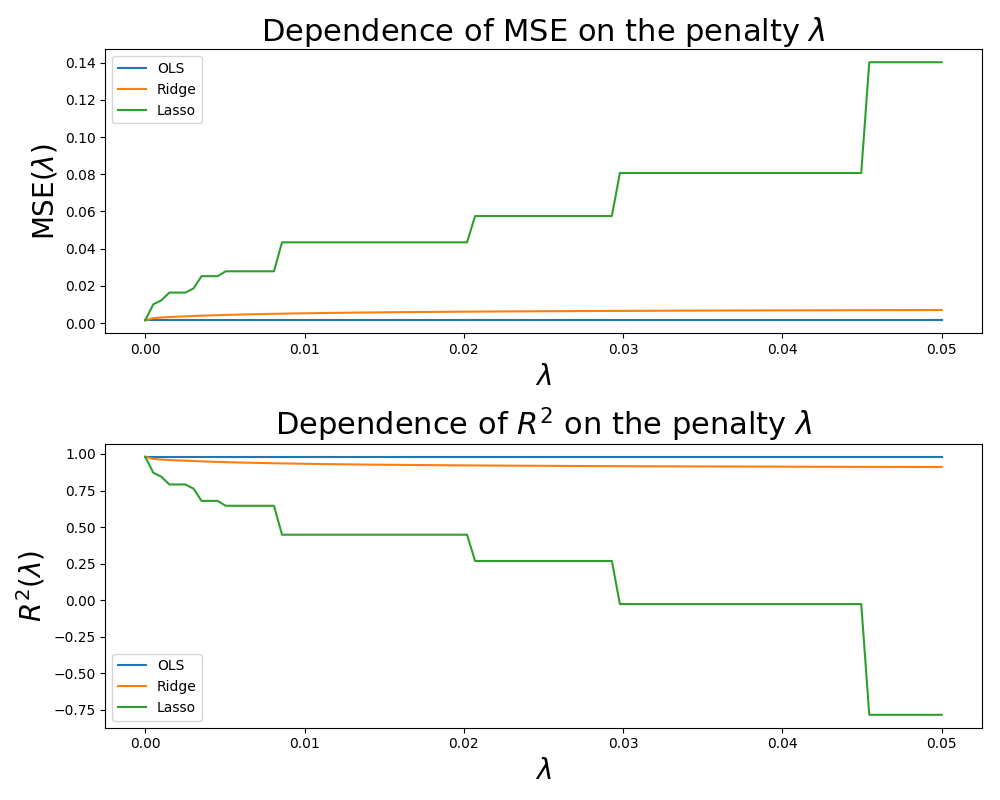
\includegraphics[scale=0.3,clip,trim={0cm 0cm 0cm 0cm}]{results/FrankeApprox/error1_deg5.png}
\caption{The dependence of MSE and \(R^2\) on the penalty regression parameter \(\lambda\).}\label{fig:error_penalty_dependence}
\end{figure}

\begin{figure}[h]
\centering
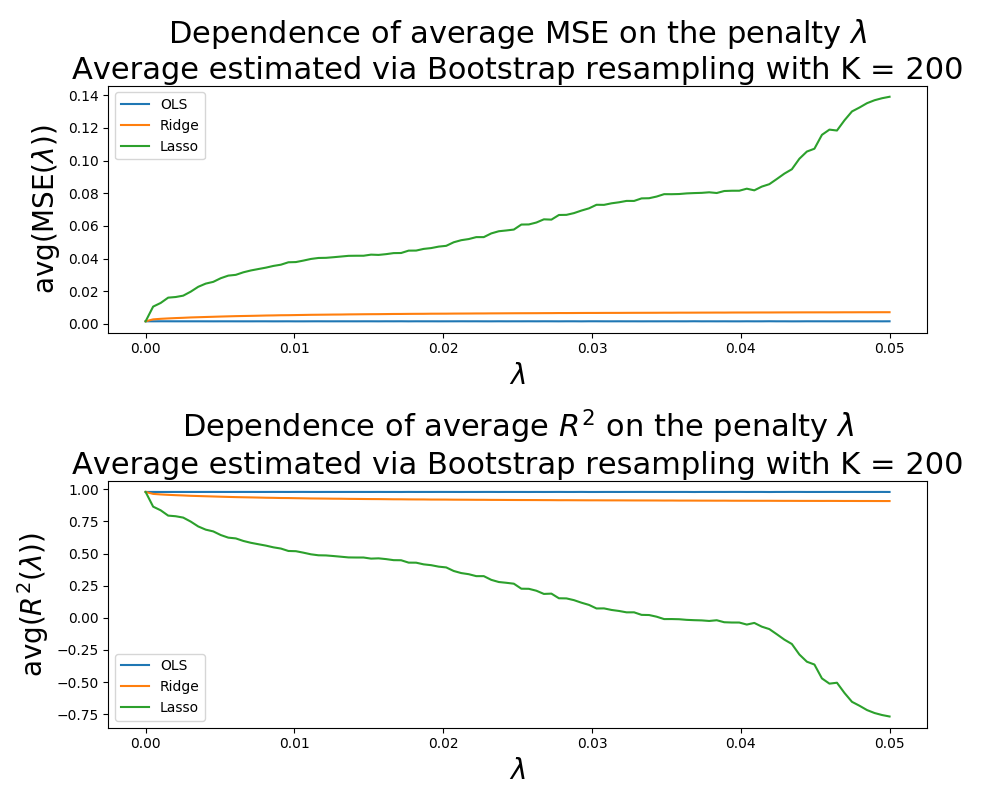
\includegraphics[scale=0.3,clip,trim={0cm 0cm 0cm 0cm}]{results/FrankeApprox/error2_deg5.png}
\caption{The dependence of average MSE and average \(R^2\) on the penalty regression parameter \(\lambda\). The averages are estimated using the Bootstrap algorithm with \(K=200\) iterations.}\label{fig:error_penalty_dependence_resampled}
\end{figure}

\begin{figure}[h]
\centering
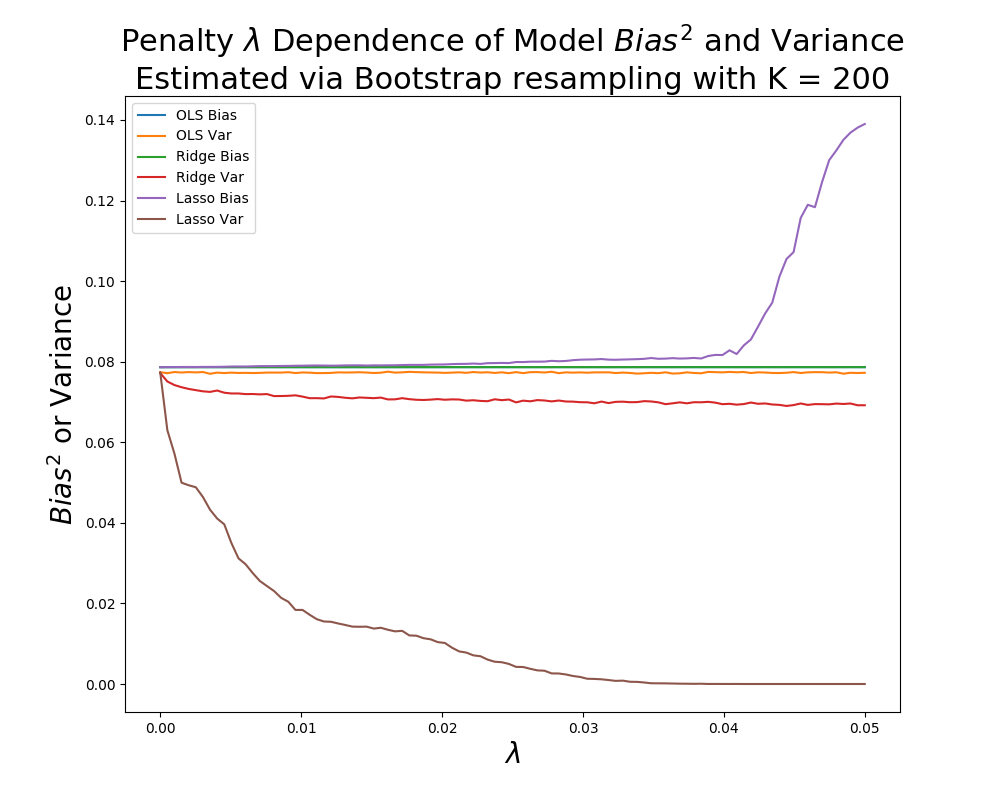
\includegraphics[scale=0.3,clip,trim={0cm 0cm 0cm 0cm}]{results/FrankeApprox/error3_deg5.png}
\caption{The dependence of estimated model \(\text{bias}^2\) and variance on the penalty regression parameter \(\lambda\). The estimations are made using the Bootstrap algorithm with \(K=200\) iterations.}\label{fig:bias_var_penalty_dependence_resampled}
\end{figure}

\subsection{Terrain Data}
A contour plot of the terrain data is included in figure \ref{fig:terrrain_data_contour} in appendix \ref{app:plots}. In addition, OLS fits using polynomials of degrees 5, 6, 7, 8, 9 and 10 are incldued in figures \ref{fig:terrrain_data_param5} through \ref{fig:terrrain_data_contour10}. From the figures it is clear that the more complex models, i.e., those of greater degree, are more realistic in terms of their curvature. The real data features a great deal of noise, which isn't captured by the parametrisations. Moreover, the sea level is heavily violated by most of the models. This is to be expected however as the models do not place any criteria on this.

In the case of the \(10^\text{th}\) degree parametrisation, the MSE and \(R^2\) scores were \(4.47664167\cdot10^3\) and \(7.39150511\cdot10^{-1}\) respectively. The size of the MSE score is most likely due to noise in the data set. As the \(R^2\) score is normalised in comparison with the MSE, it does not show the same ridiculous numbers. Nonetheless, a \(R^2\) of about 0.74 is not very impressive to say the least. The parametrisations are great for capturing the major structures in the data, but fail to reproduce the data.
\section{Discussion}
The analysis of Franke's function illuminated how stable the penalty dependence of Ridge regression is compared to Lasso regression. This is likely due to Lasso's unique ability of completing freezing out some parameters, while Ridge on the other hand changes slowly with respect to \(\lambda\). 

The \(10^\text{th}\) degree OLS parametrisation of the terrain data showed that these kinds of methods are very adaptible for describing the large structures and shapes of noisy data such as the terrain data. However, in order to reproduce the terrain, other methods should be used instead.
\section{Conclusion}
Linear regression proved a fair condidate for parametrising surfaces using polynomial models. While the parametrisations are unable to fully repoduce the underlying surfaces, they do describe their overaching shape. This is useful in cases when detailed maps are uneccessary, and only a major description is needed.

\nocite{book}\nocite{project}
\bibliographystyle{plain}
\bibliography{references}
\clearpage
\appendix
\section{Plots}\label{app:plots}
\begin{figure}[h]
\centering
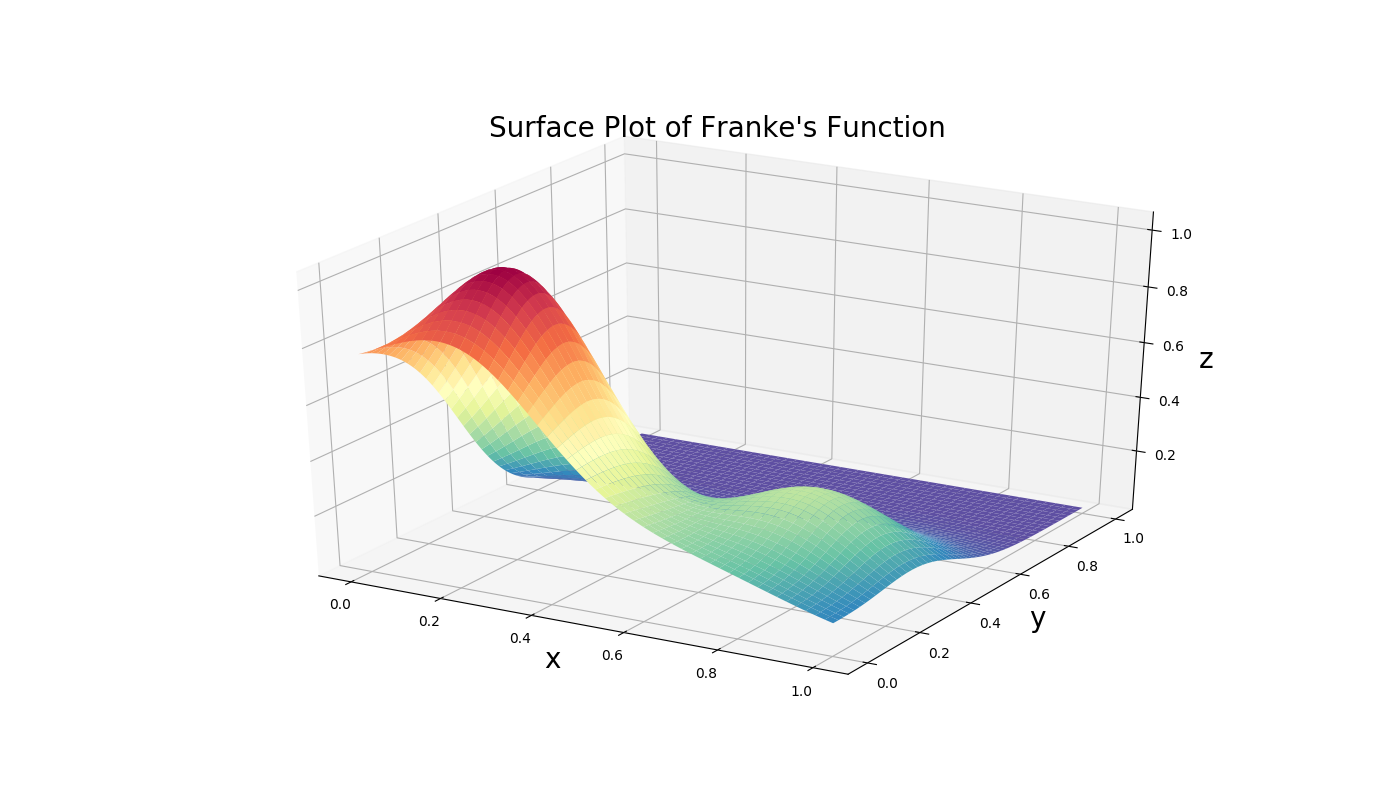
\includegraphics[scale=0.25,clip,trim={8cm 2cm 4cm 1cm}]{results/FrankeApprox2/exact_surface.png}
\caption{Surface plot of Franke's function for \((x,y)\in[0,0]\times[1,1]\).}\label{fig:franke_function}
\end{figure}

\begin{figure}[h]
\centering
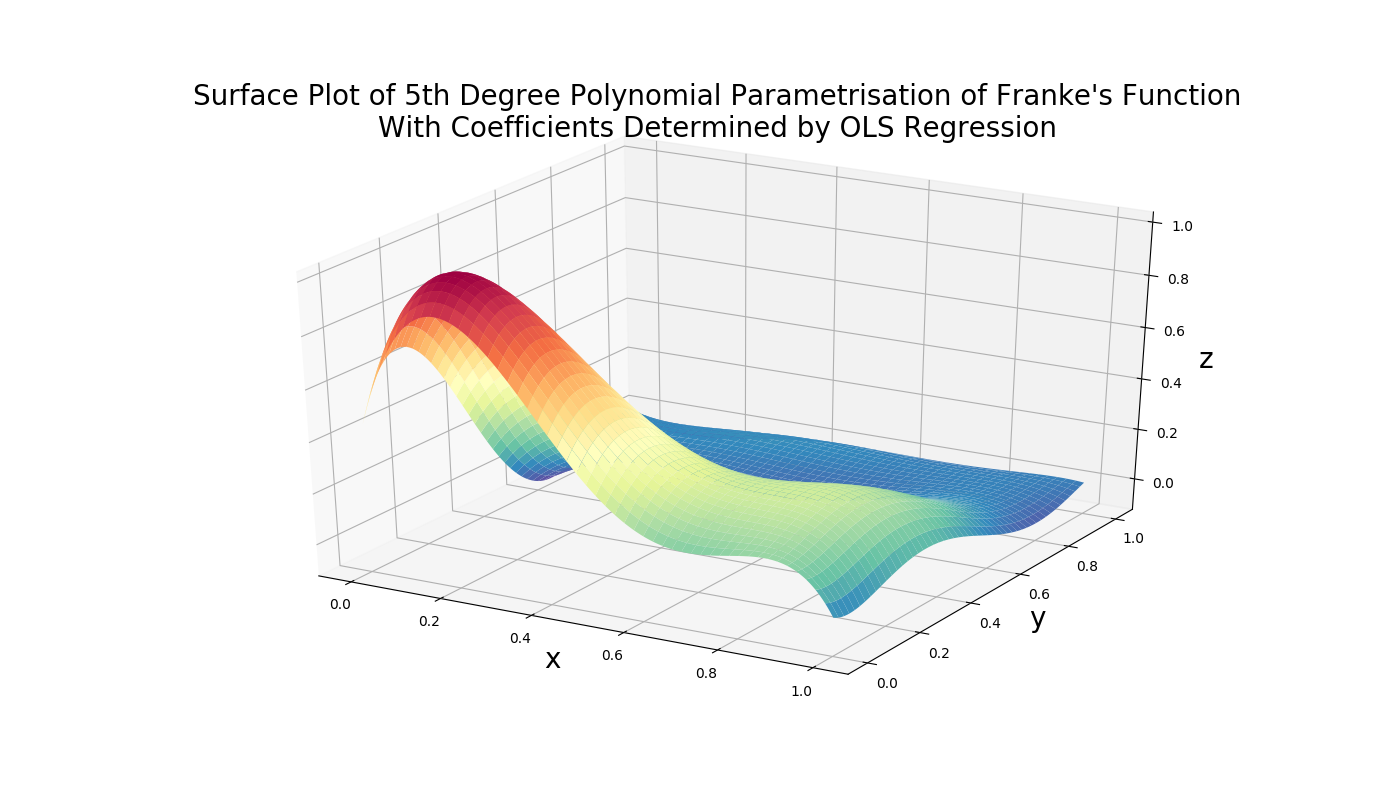
\includegraphics[scale=0.25,clip,trim={4cm 2cm 4cm 1cm}]{results/FrankeApprox2/surface_deg5_OLS.png}
\caption{Surface plot of a \(5^{\text{th}}\) degree polynomial parametrisation of Franke's function for \((x,y)\in[0,0]\times[1,1]\), with term coefficients determined via Ordinary Least Squares regression analysis.}\label{fig:franke_parametrisation_ols}
\end{figure}

\begin{figure}[h]
\centering
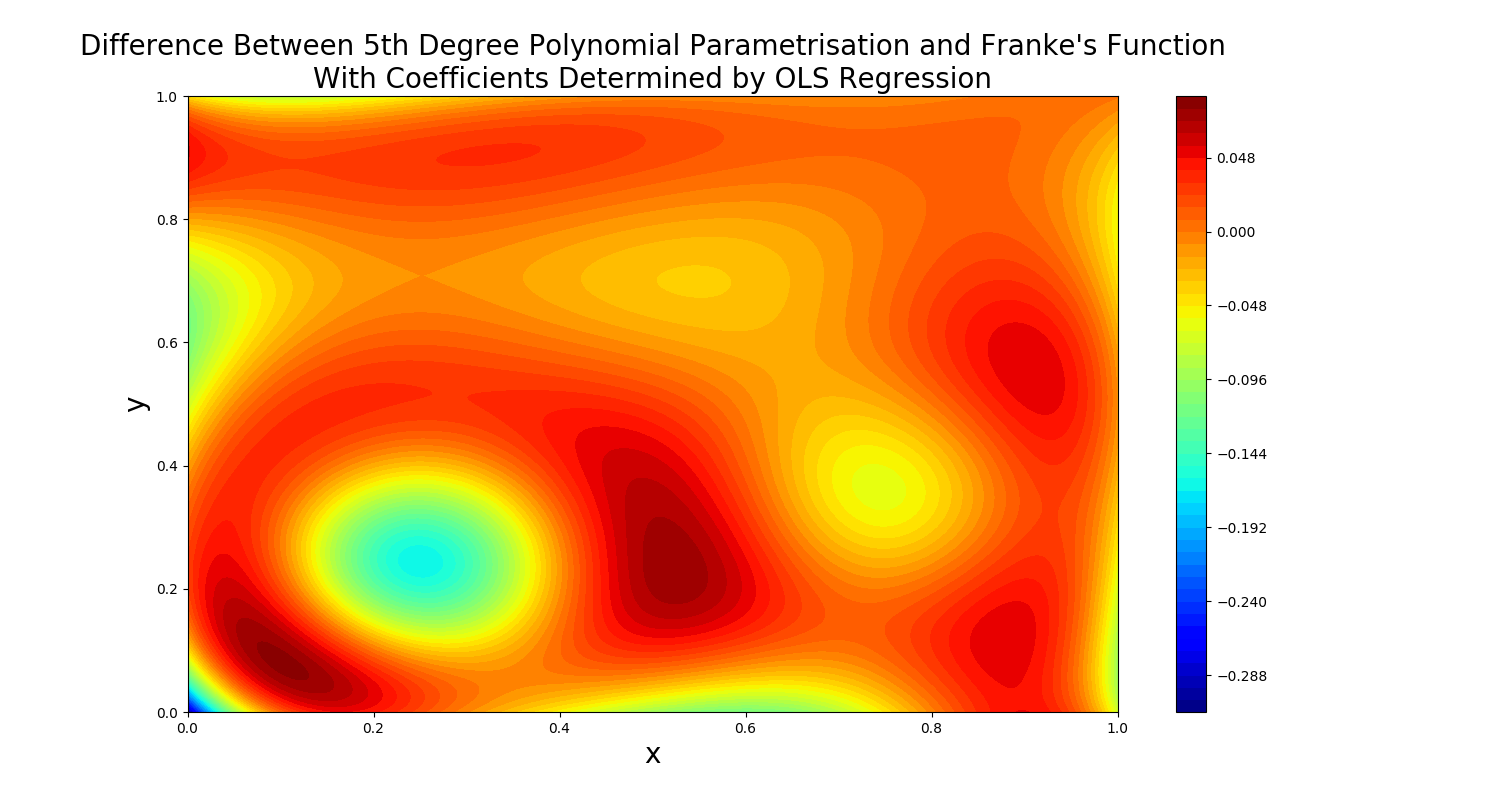
\includegraphics[scale=0.25,clip,trim={2cm 0cm 4cm 0cm}]{results/FrankeApprox2/diff_deg5_OLS.png}
\caption{Contour plot of the difference between a \(5^{\text{th}}\) degree polynomial parametrisation of Franke's function and Franke's function for \((x,y)\in[0,0]\times[1,1]\), with term coefficients determined via Ordinary Least Squares regression analysis.}\label{fig:franke_difference_ols}
\end{figure}

\begin{figure}[h]
\centering
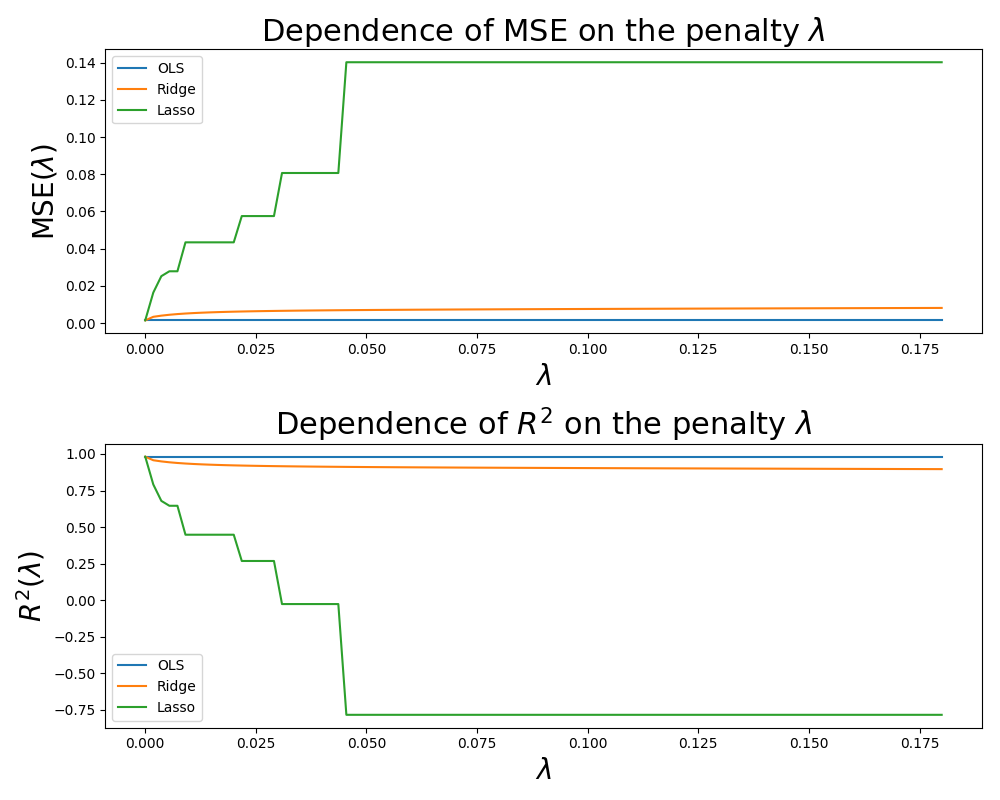
\includegraphics[scale=0.3,clip,trim={0cm 0cm 0cm 0cm}]{results/FrankeApprox3/error1_deg5.png}
\caption{The dependence of MSE and \(R^2\) on the penalty regression parameter \(\lambda\).}\label{fig:error_penalty_dependence2}
\end{figure}

\begin{figure}[h]
\centering
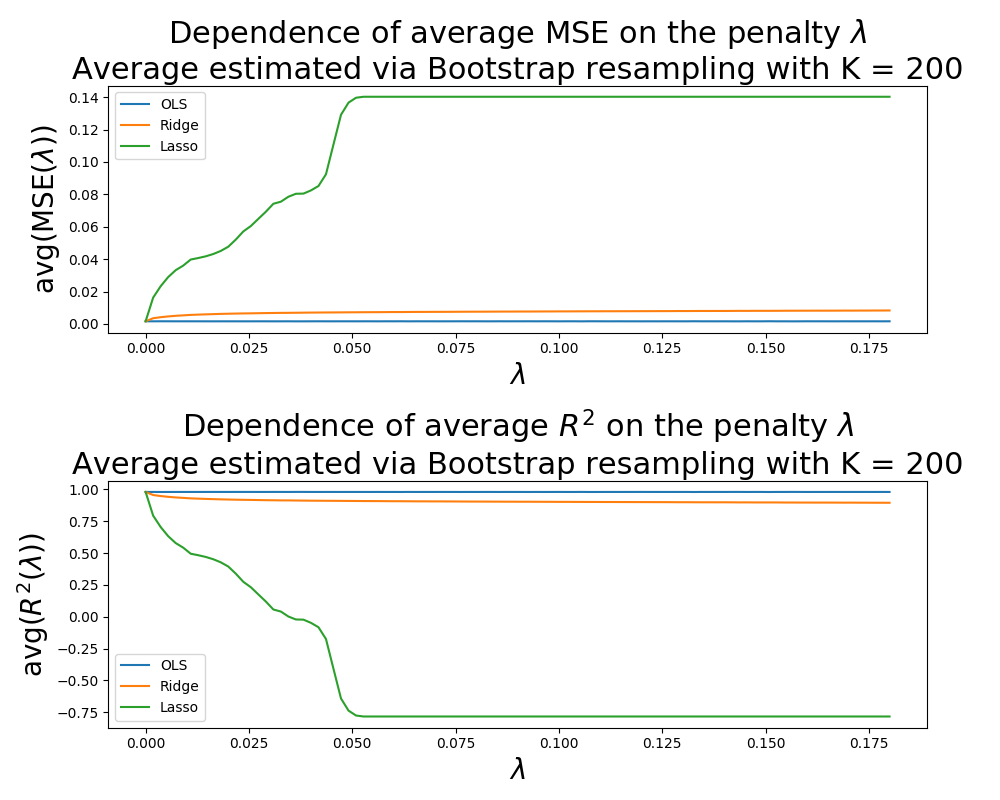
\includegraphics[scale=0.3,clip,trim={0cm 0cm 0cm 0cm}]{results/FrankeApprox3/error2_deg5.png}
\caption{The dependence of average MSE and average \(R^2\) on the penalty regression parameter \(\lambda\). The averages are estimated using the Bootstrap algorithm with \(K=200\) iterations.}\label{fig:error_penalty_dependence_resampled2}
\end{figure}

\begin{figure}[h]
\centering
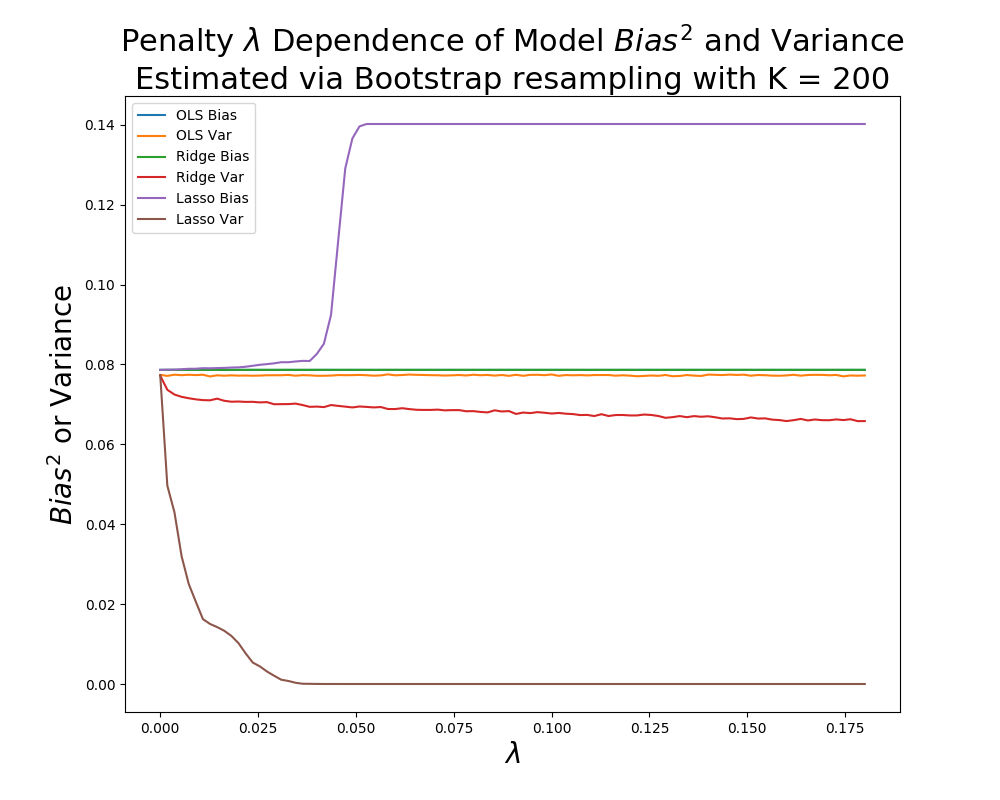
\includegraphics[scale=0.3,clip,trim={0cm 0cm 0cm 0cm}]{results/FrankeApprox3/error3_deg5.png}
\caption{The dependence of estimated model \(\text{bias}^2\) and variance on the penalty regression parameter \(\lambda\). The estimations are made using the Bootstrap algorithm with \(K=200\) iterations.}\label{fig:bias_var_penalty_dependence_resampled2}
\end{figure}

\begin{figure}[h]
\centering
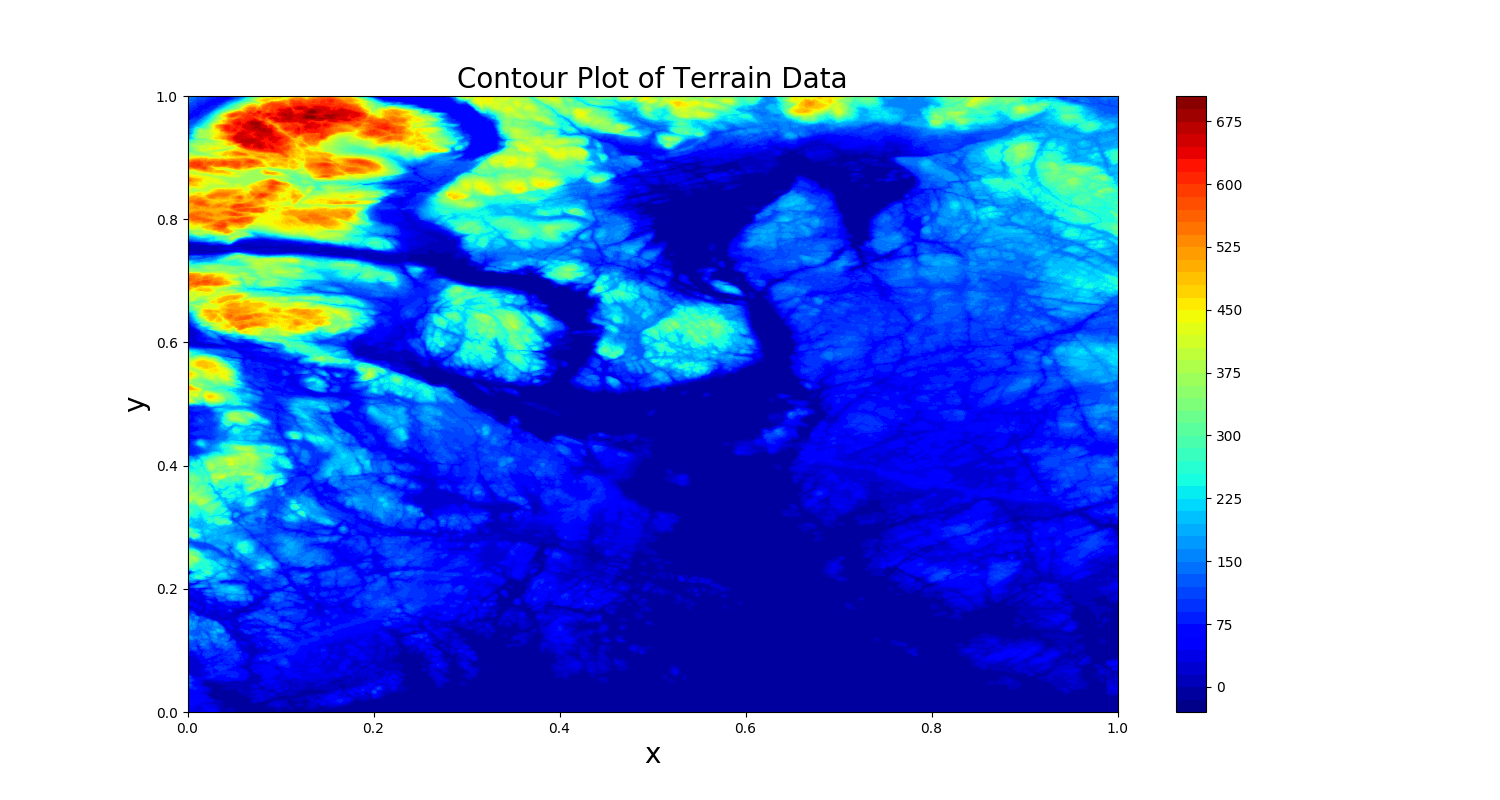
\includegraphics[scale=0.2,clip,trim={0cm 0cm 0cm 0cm}]{results/TerrainApprox/terrain_contour.png}
\caption{Contour plot of the terrrain data set.}\label{fig:terrrain_data_contour}
\end{figure}

\begin{figure}[h]
\centering
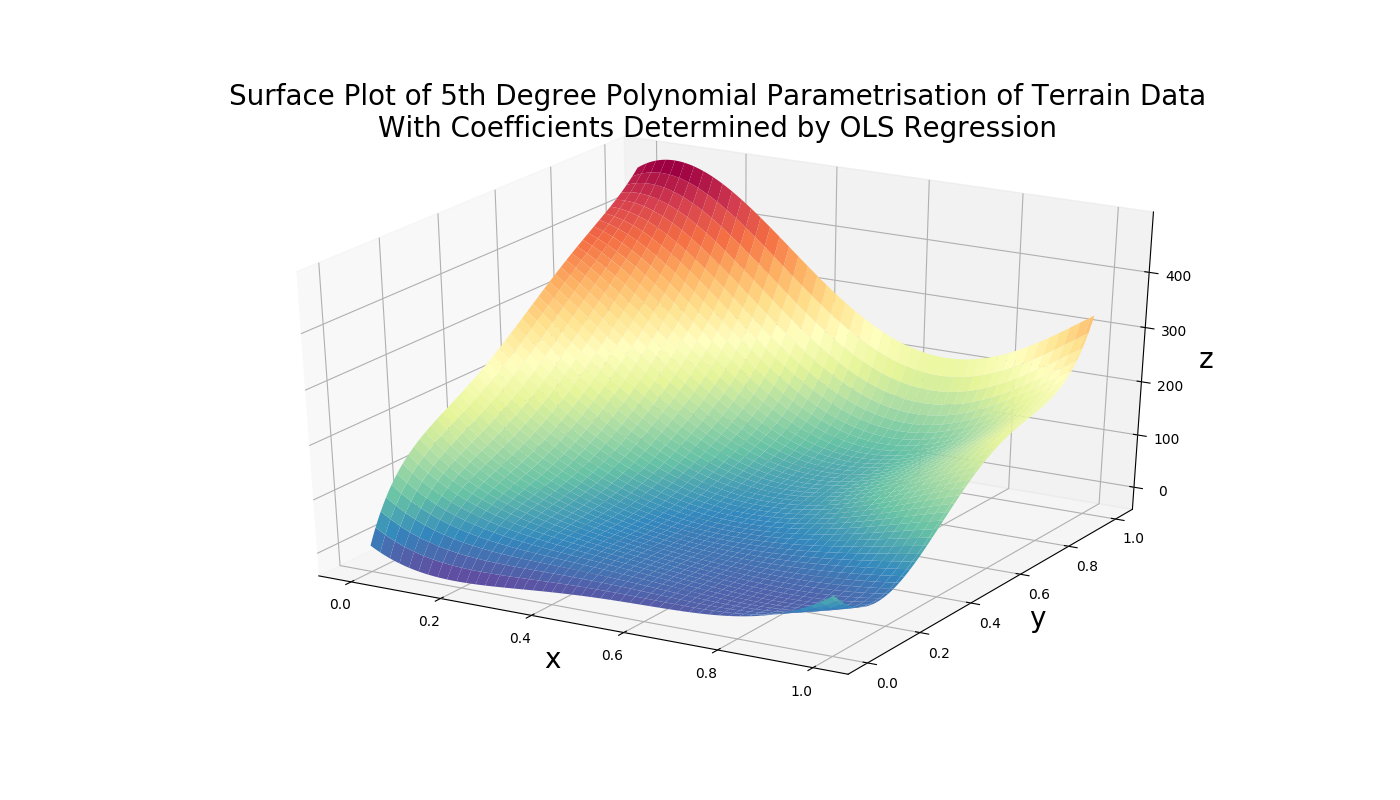
\includegraphics[scale=0.25,clip,trim={4cm 2cm 4cm 1cm}]{results/TerrainApprox/surface_deg5_OLS.png}
\caption{Surface plot of a polynomial parametrisation of the terrrain data set of degree 5.}\label{fig:terrrain_data_contour}
\end{figure}
\newpage

\begin{figure}[h]
\centering
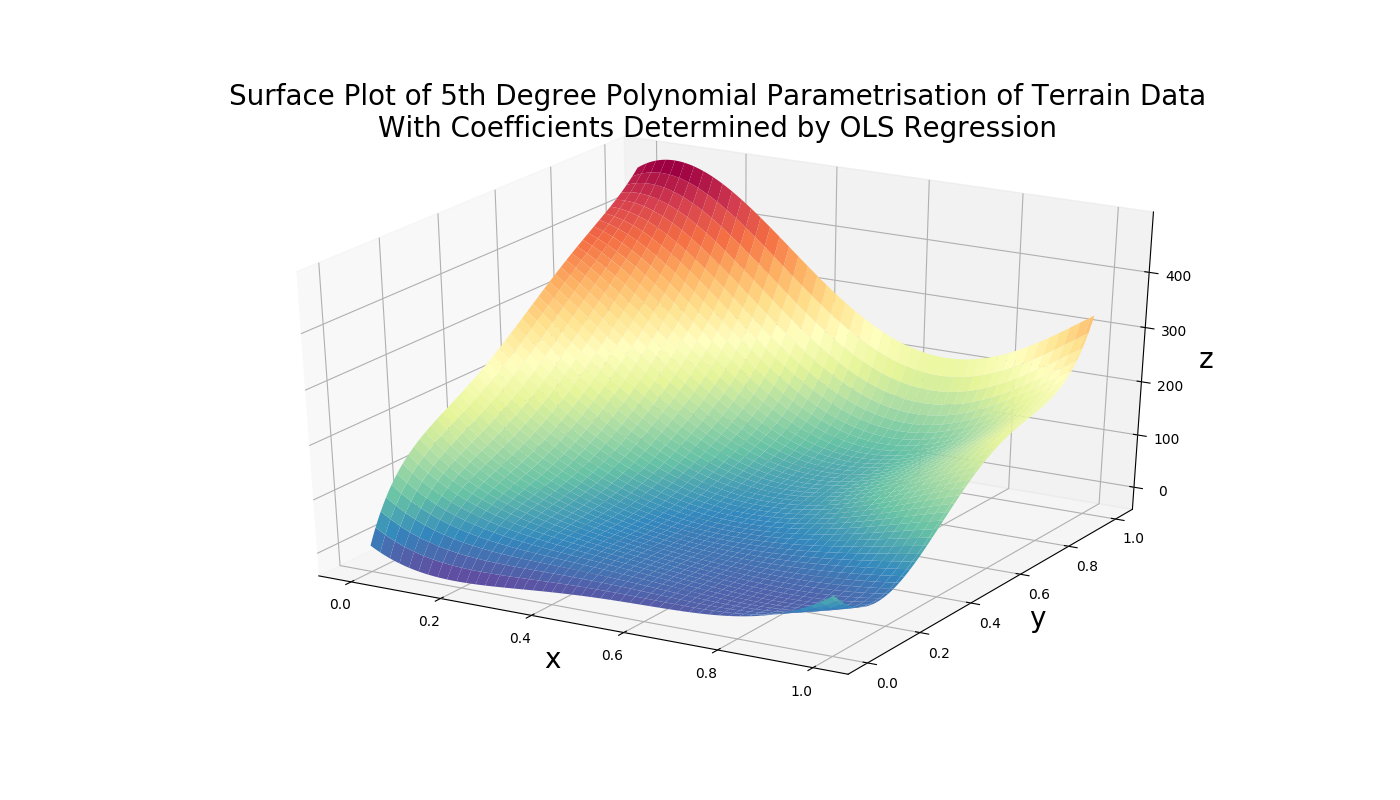
\includegraphics[scale=0.25,clip,trim={4cm 2cm 4cm 1cm}]{results/TerrainApprox/surface_deg5_OLS.png}
\caption{Surface plot of a polynomial parametrisation of the terrrain data set of degree 5.}\label{fig:terrrain_data_param5}
\end{figure}

\begin{figure}[h]
\centering
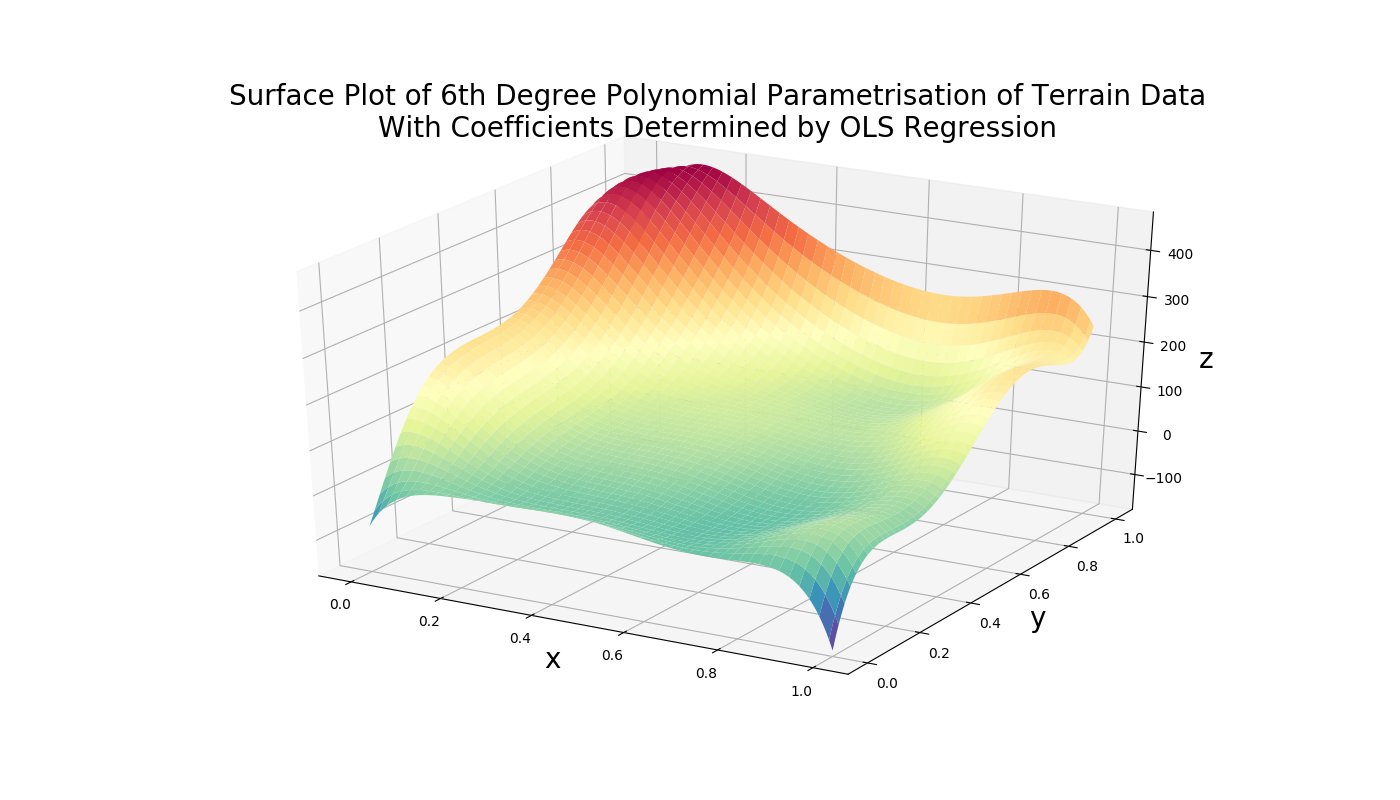
\includegraphics[scale=0.25,clip,trim={4cm 2cm 4cm 1cm}]{results/TerrainApprox2/surface_deg6_OLS.png}
\caption{Surface plot of a polynomial parametrisation of the terrrain data set of degree 6.}\label{fig:terrrain_data_contour6}
\end{figure}

\begin{figure}[h]
\centering
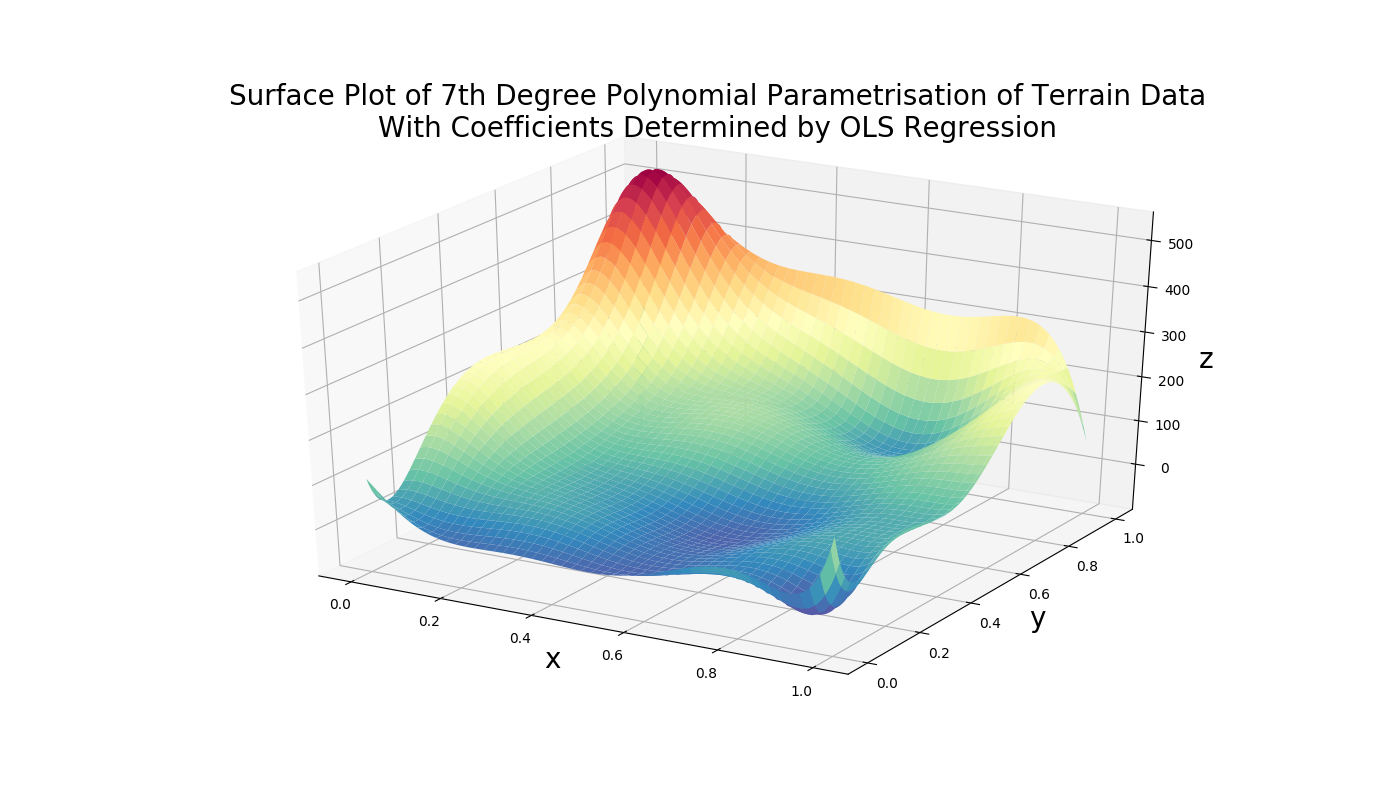
\includegraphics[scale=0.25,clip,trim={4cm 2cm 4cm 1cm}]{results/TerrainApprox3/surface_deg7_OLS.png}
\caption{Surface plot of a polynomial parametrisation of the terrrain data set of degree 7.}\label{fig:terrrain_data_contour7}
\end{figure}

\begin{figure}[h]
\centering
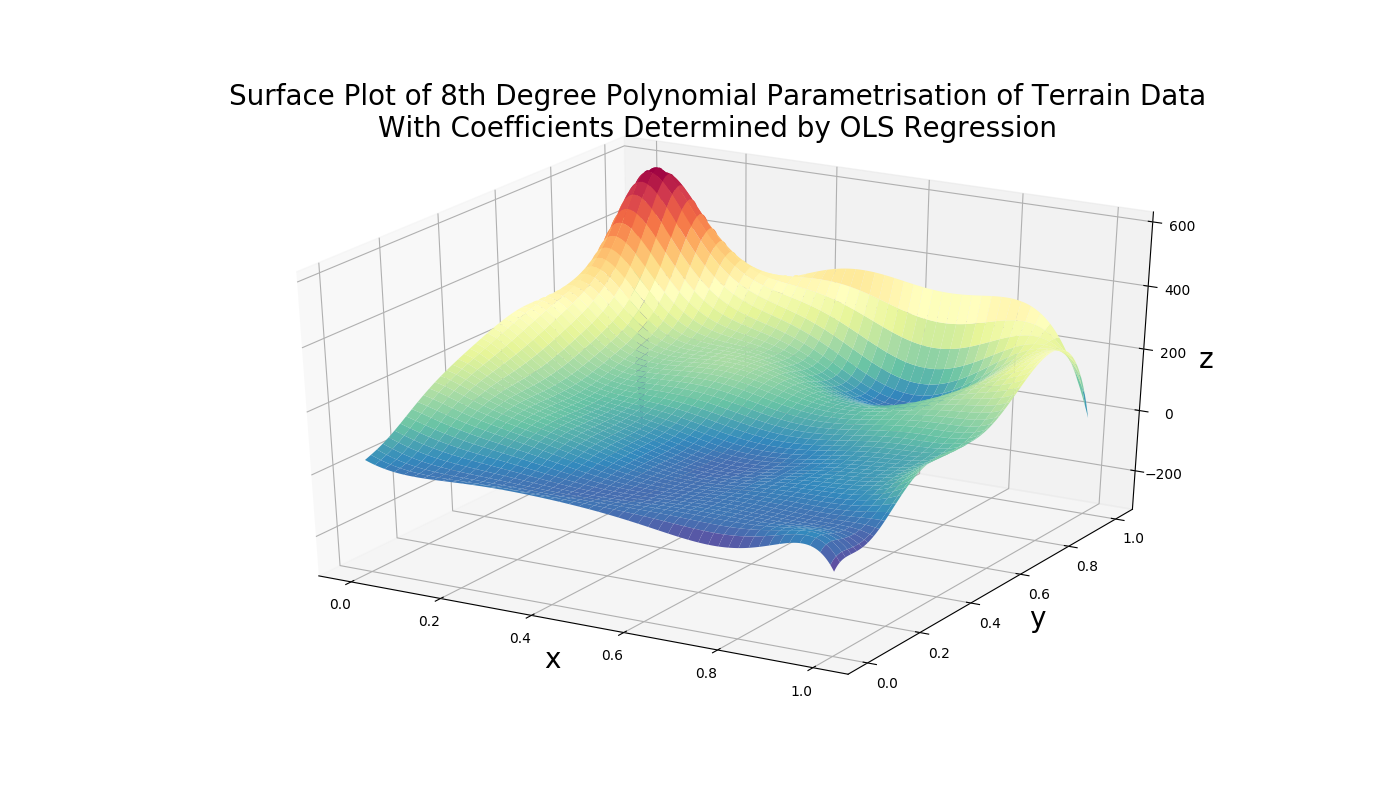
\includegraphics[scale=0.25,clip,trim={4cm 2cm 4cm 1cm}]{results/TerrainApprox4/surface_deg8_OLS.png}
\caption{Surface plot of a polynomial parametrisation of the terrrain data set of degree 8.}\label{fig:terrrain_data_contour8}
\end{figure}

\begin{figure}[h]
\centering
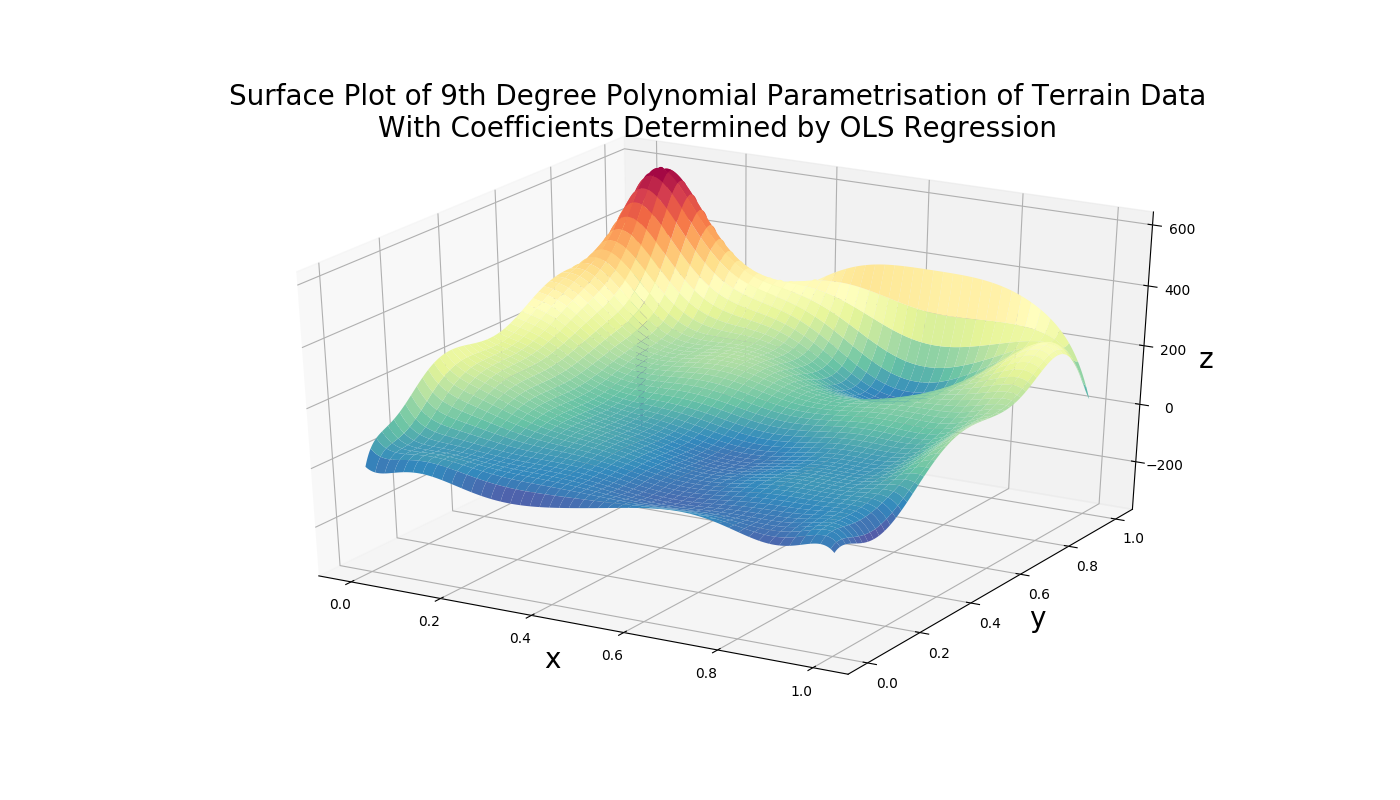
\includegraphics[scale=0.25,clip,trim={4cm 2cm 4cm 1cm}]{results/TerrainApprox5/surface_deg9_OLS.png}
\caption{Surface plot of a polynomial parametrisation of the terrrain data set of degree 9.}\label{fig:terrrain_data_contour9}
\end{figure}

\begin{figure}[h]
\centering
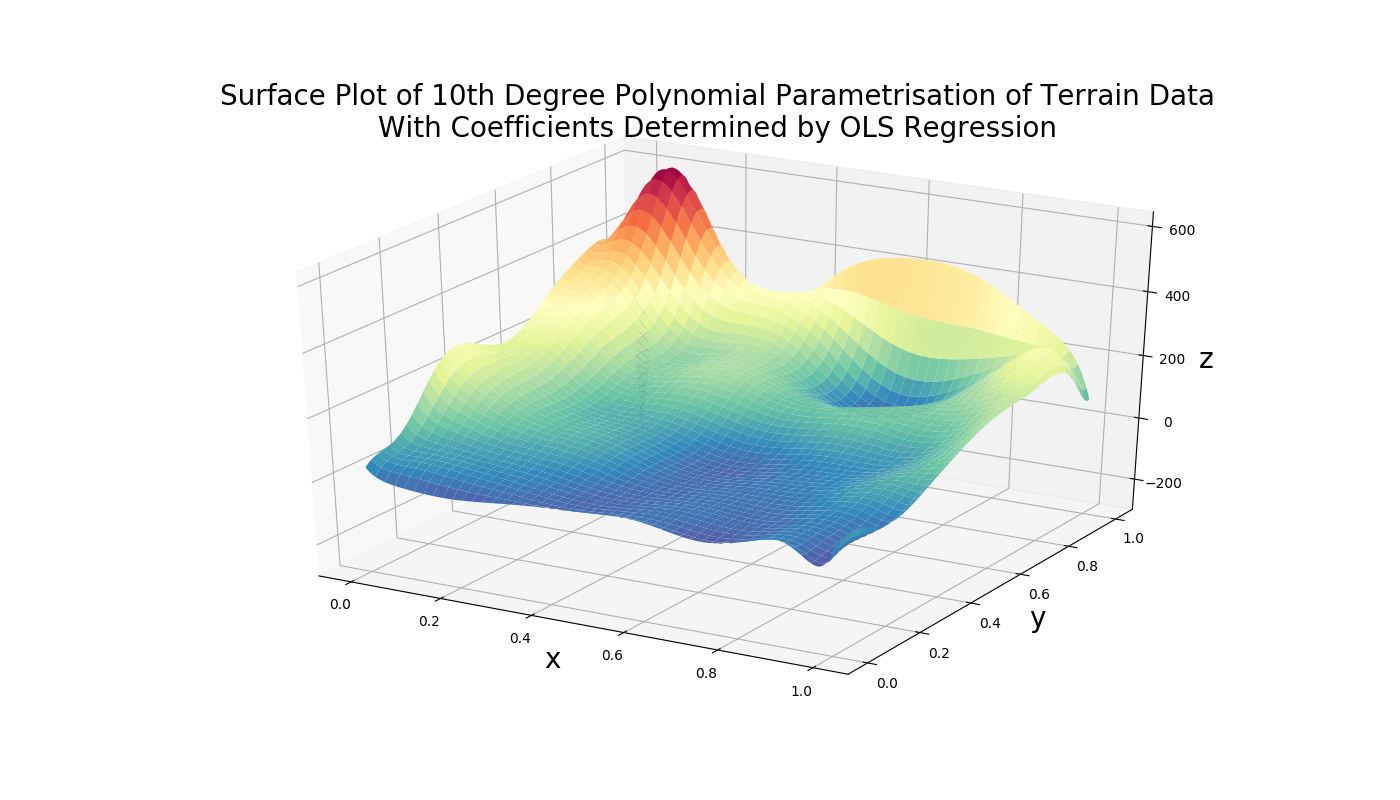
\includegraphics[scale=0.25,clip,trim={4cm 2cm 4cm 1cm}]{results/TerrainApprox6/surface_deg10_OLS.png}
\caption{Surface plot of a polynomial parametrisation of the terrrain data set of degree 10.}\label{fig:terrrain_data_contour10}
\end{figure}
\clearpage
~
\onecolumngrid
\section{Equations}\label{app:list_of_eq}
Franke's test function is the following weighted sum of four bivariate gaussian curves:
\begin{equation}\label{eq:appendix:Franke:Franke_function}
f(x,y)=\frac{3}{4}e^{-\frac{(9x-2)^2}{4}-\frac{(9y-2)^2}{4}}+\frac{3}{4}e^{-\frac{(9x+1)^2}{49}-\frac{(9y+1)^2}{10}}
+\frac{1}{2}e^{-\frac{(9x-7)^2}{4}-\frac{(9y-3)^2}{4}}-\frac{1}{5}e^{-(9x-4)^2-(9y-7)^2}
\end{equation}
The explicit expression for the \(5^{\text{th}}\) degree polynomial parametrisation used in the analysis of Franke's function is given below. Note that the ordering of the terms is important. To emphasise the difference between the terms, extra vertical spacing is added so that each line consists of same-degree terms (for the sake of clarity).
\begin{align}\label{eq:appendix:Franke:general_5th_order_model}
z(x,y)=\ &\beta_0+\nonumber\\
         &\beta_1x      +\beta_2y+\nonumber\\
         &\beta_3x^2    +\beta_4xy      +\beta_5y^2+\nonumber\\
         &\beta_6x^3    +\beta_7x^2y    +\beta_8xy^2      +\beta_9y^3+\nonumber\\
         &\beta_{10}x^4 +\beta_{11}x^3y +\beta_{12}x^2y^2 +\beta_{13}xy^3   +\beta_{14}y^4+\nonumber\\
         &\beta_{15}x^5 +\beta_{16}x^4y +\beta_{17}x^3y^2 +\beta_{18}x^2y^3 +\beta_{19}xy^4+\beta_{20}y^5
\end{align}
Hence, the entire model consists of 21 parameters: \(\beta_0,\ldots,\beta_{20}\).
\twocolumngrid


\end{document}
